\documentclass[a4paper,parskip=half,ibliography=totocnumbered,titlepage]{scrartcl}

\usepackage[T1]{fontenc}  
\usepackage[utf8]{inputenc}
\usepackage[ngerman]{babel}
\renewcaptionname{ngerman}{\figurename}{Abb.}

\usepackage{multicol}         
\usepackage{mathtools}       
\usepackage{amssymb}
\usepackage{listings}      
\usepackage{csquotes}
\usepackage{pifont}

% Tabellen
\usepackage{booktabs}
\usepackage{multirow}
\usepackage{multicol}

\usepackage{tocloft}
\renewcommand{\cftfigpresnum}{Abb. }
\settowidth{\cftfignumwidth}{Abb. 10\quad}


\usepackage{ifthen}
\newcommand{\forloop}[5][1]{%
\setcounter{#2}{#3}%
\ifthenelse{#4}{#5\addtocounter{#2}{#1}%
\forloop[#1]{#2}{\value{#2}}{#4}{#5}}%
{}}

\newcounter{crcounter}

\newcommand{\compensaterule}[1]{%
\forloop{crcounter}{1}{\value{crcounter} < #1}%
{\vspace*{-\aboverulesep}\vspace*{-\belowrulesep}}}

\newcommand{\multirowbt}[3]{\multirow{#1}{#2}%
{\compensaterule{#1}#3}}


% bibtex
\usepackage[natbib,bibencoding=auto,style=authoryear,backend=biber]{biblatex}
\bibliography{references.bib}
\DeclareLanguageMapping{ngerman}{ngerman-apa}


%Schusterjungen und Hurenkinder
\clubpenalty = 10000
\widowpenalty = 10000

%Farbnamen benutzen
\usepackage[usenames,dvipsnames]{color}

\definecolor{black}{gray}{0} % Umdefinition der Farbe black, falls noetig (0=schwarz, 1=weiss)
\definecolor{dblue}{rgb}{0.1,0.2,0.6} % Dunkelblau, fuer Hyperlinks
\definecolor{lgray}{gray}{0.9} % Hellgrau, fuer Tabellen (0=schwarz, 1=weiss)
\usepackage[hyperfootnotes=false,colorlinks=true,linkcolor=black,citecolor=dblue,urlcolor=dblue]{hyperref} 

\usepackage{setspace}

\usepackage{enumitem}
\setlist{noitemsep} % or \setlist{noitemsep} to leave space around whole list

% \begin{enumerate}[label=(\roman{*})]

\newcommand{\HRule}[1]{\rule{\linewidth}{#1}} 	% Horizontal rule

\makeatletter							% Title
\def\printtitle{%						
    {\centering \@title\par}}
\makeatother									

\makeatletter							% Author
\def\printauthor{%					
    {\centering \large \@author}}				
\makeatother							

\usepackage{lastpage}
\usepackage{fancyhdr}
\pagestyle{fancy}
\fancyhf{}
\renewcommand{\footrulewidth}{0.5pt}
\renewcommand{\headrulewidth}{0.5pt}


% ------------------------------------------------------------------------------
% Metadata (Change this)
% ------------------------------------------------------------------------------

%Kopf- und Fußzeile, jeweils links und rechts
\fancyhead[L]{Dokumentation}
\fancyhead[R]{A.R.C.S.}
\fancyhead[L]{Projekt C}
\fancyfoot[R]{Seite \thepage\ von~\pageref{LastPage}}

%Titelblat
\title{\normalsize \textsc{Dokumentation Projekt C} 	% Subtitle of the document
		 	\\[2.0cm]													% 2cm spacing
            \HRule{0.5pt} \\ [0.5cm]										% Upper rule + 0.5cm spacing
			\LARGE \textbf{\uppercase{A.R.C.S - Android Rubik's Cube Solver}}	% Title
			\HRule{0.5pt} \\ [0.5cm]								% Lower rule + 0.5cm spacing
			\large Stephan Halbritter (Matr.-Nr.: 2093970)\\
      Colin Sames (Matr.-Nr.: 2093044)\\
		}

\author{Betreuer: Prof.~Dr.~Plaß\\
    Media Systems (B.Sc.)\\
    Hochschule für Angewandte Wissenschaften Hamburg\\
}


\begin{document}
% ------------------------------------------------------------------------------
% Maketitle
% ------------------------------------------------------------------------------
\thispagestyle{empty}				% Remove page numbering on this page

\printtitle									% Print the title data as defined above
  	\vfill
\printauthor								% Print the author data as defined above
\newpage

\begin{abstract}
Vermutlich brauchen wir hierfür kein Abstrakt, aber ich lasse es erstmal drin.
\end{abstract}

\tableofcontents
\newpage

\section{Beispielkrams}
Beispielabschnitt, in den ich die am meisten benutzen Auszeichnungen nutze:

\emph{Betonung, kursiv}

\begin{figure}[ht!]
    \centering
    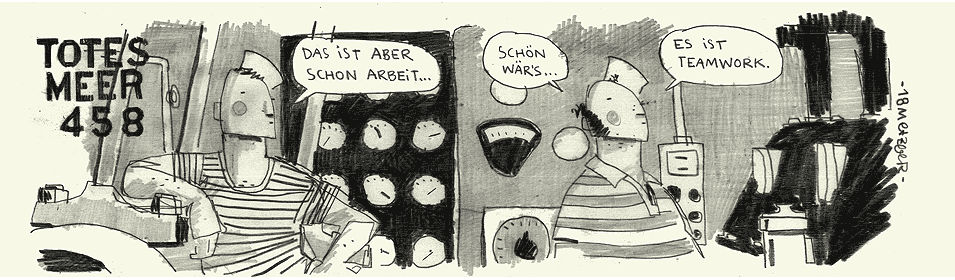
\includegraphics[width=\textwidth]{pics/test.png}
    \caption{Eine Beispielunterschrift unter einem Beispielbild}
    \label{fig:test}
\end{figure}

Benötigte Pakete:
\begin{itemize}

  \item texlive-bibtexextra
  \item texlive-core
  \item texlive-latexextra
  \item texlive-science
  \item Alle Pakete gibt es auch für Debian
  \item (für eine nummerierte Liste nutzt man \emph{enumerate} anstelle von
    \emph{itemize})

\end{itemize}

Technische Begriffe\footnote{Das ist eine Fußnote} oder Code im Fließtext:
\texttt{com.github.sgelb.arcs}

Auf das Label aus der Abbildung kann man sich beziehen, die Nummerierung
geschieht automatisch: siehe Abbildung~\ref{fig:test}).


\textbf{Codeblock:}

\begin{lstlisting}
connect(ui->nextBtn, &QPushButton::clicked, this,
        &MainWindow::nextTrack);
\end{lstlisting}

Am Ende noch eine URL, die sich natürlich im pdf Anklicken lässt:
\url{http://qt-project.org/doc/qt-5/qmediaplayer.html}

Mein workflow sieht in der Regel so aus, dass ich aus vim heraus das pdf
erstelle:

\texttt{:!pdflatex \%}\footnote{das Ausrufezeichen ruft einen
externen Befehl auf, das Prozentzeichen steht für das gesamte Dokument}

Einmal erstellt, öffne ich das pdf und da die meisten pdf-Viewer Änderungen
erkennen, wird das angezeigte pdf bei jeder Neugenerierung aktualisiert.
Manchmal sind zwei oder drei Aufrufe von \texttt{pdflatex} nötig, um
Inhaltsverzeichnis etc korrekt zu erstellen.

Quellenangaben sind in \texttt{references.bib} im BibText-Format
\citep{wiki:bibtex} gelistet und können mit dem entsprechen Befehl eingefügt
werden. Das ist ein absolutes Killerfeature von Tex, aber werden wir nicht
brauchen, darum gehe ich da nicht weiter drauf ein. Geiler Scheiß:
\url{http://www.rtwilson.com/academic/autozotbib},
\url{http://manas.tungare.name/software/isbn-to-bibtex/} und
\url{http://lead.to/amazon/en/?key=OpenCV&si=owb&op=bt&bn=&so=ta&ht=de}




\section{Einleitung}  % sgelb 0%
\subsection{Idee}  % sgelb 0%

\section{Umsetzung}  % sgelb 0%
\subsection{Bibliotheken und Tools}  % colin 0%
In diesem Kapitel werden die in diesem Projekt verwendeten Bibliotheken und Hilfswerkzeuge
vorgestellt, ohne deren Hilfe das Projekt kaum Umsetzbar gewesen wäre.
\subsubsection{OpenCV}  % 0%
OpenCV ist eine Bibliothek, die eine große Fülle an Funktionen, unter Anderem zur Bildbearbeitung, zur Verfügung stellt.
Daher war sie für dieses Projekt unverzichtbar. Gerade Farberkennung eines mit dem Smartphone aufgenommenen Bildes
war mittels OpenCV um ein vielfaches einfacher zu implementieren.
\subsubsection{Eclipse}  % 0%
Als IDE haben wir Eclipse Juno verwendet, da Juno kompatibler mit der Einbindung der Android Plugins war.
Mittels des Android SDK Manager konnte man die APIs der jeweiligen Android Version einfach einbinden.
OpenCV, ADT und NDK wurden seperat dem Projekt hinzugefügt.
Eclipse bietet zudem auch die Möglichkeit sehr einfach Tests mittels JUnit zu schreiben.
Gerade Tests sind sehr wichtig für dieses Projekt gewesen, in dem sich durch Änderungen Fehler aller Art
entwickeln konnten. Das diese Fehler überhaupt vorhanden sind, ließ sich durch die TestCases gut identifizieren.
\subsubsection{Git}  % 0%
Als Versionsverwaltungssoftware haben wir Git gewählt. Auf GitHub haben wir ein Repository angelegt.
Die Branchstruktur liegt dieser Idee zugrunde: <LINK HIER ICH FIND DEN GERADE NICHT>
Git bietet zudem den Vorteil, dass alle Mitglieder des Projekts Zugriff auf den Code haben und
seperat daran Arbeiten konnten.
Wir haben bewusst auf das EGit Plugin für Eclipse verzichtet, da dieses mehr Probleme schafft als es diese löst.
Stattdessen haben wir traditionell die Konsole benutzt.
\subsubsection{ADT/NDK}  % 0%
Die Android Development Tools bieten eine Vielzahl an GUI Funktionen zur Entwicklung von Android Apps unter Eclipse.
KP man, LATER
\subsubsection{Java}  % 0%
Als Programmiersprache wurde Java benutzt. Java bietet sich sehr für App Entwicklung an, da auch OpenCV
damit kompatibel ist und, App Entwicklung an sich, auch ohne Zuzug von OpenCV, mittels Java realisierbar
ist.

\subsection{Gestaltung}  % sgelb 0%
\subsection{Arbeitsprozess}  % sgelb 0%

\section{Benutzerhandbuch}  % colin 0%
Die App A.R.C.S. ist eine App zur Lösung eines Rubiks Cube.
Nach dem Starten der App bekommt der User beim Queer halten des Smartpones links das Kamerafeld und rechts
eine Beschreibung sowie einige Funktionen zu sehen. Auf dem Kamerafeld links befinden sich 9 Quadrate.
Der User hat die Wahl den Würfel mittels der Kamera einzulesen, oder manuell. Möchte er dies automatisch tun,
so hält er den Würfel in die Kamera und achtet darauf, dass sich jedes Feld auf dem Würfel in einem Quadrat
auf dem Bildschirm befindet. Wie der User den Würfel halten muss, wird mit einer Beschreibung rechts verdeutlicht.
Zudem befindet sich über den 9 Quadraten ein Farblick makierter Strich, der zeigt, welche Farbe (mittleres Feld
des Würfels) oben liegen soll. Das Mittlere der 9 Quadrate ist auch Farblich markiert. So kann eine eindeutige
Position des Würfels ermittelt werden. Hat der User den Würfel richtig positioniert, so kann er rechts auf einen
Button klicken, der die Farben des Würfels erkennt. Die Quadrate bekommen nun die Farben der erkannten Felder.
Sollte eine Farbe nicht richtig erkannt worden sein, so kann er entweder erneut den Button betätigen oder manuell
die Farbe ändern indem er auf das Quadrat klickt. Der User bekommt nun eine Liste mit 9 Farben aus der er die
gewünscht Farbe selektieren kann. Stimmen alle Farben, so kann der User auf einen Butten mit einem "weiter"
Pfeil drücken. Nun bekommt er die nächste Seite des Würfels. Die Hinweise zur richtigen Ausrichtung des Würfels
sind für jede Seite angepasst. Möchte der User eine Seite zurück gehen, so gibt es auch analog zum "weiter" Button
auch einen "zurück" Button. Die vorher eingelesenen Farben sind dort noch gespeichert und können editiert werden.
Nachdem der User alle Seiten eingelesen hat, kann er den Würfel mittels eines Buttons auf der rechten Seite lösen
lassen. Wurde der Würfel nicht rictig eingelesen, so bekommt der User einen Hinweis das es z.B. nicht genau 9
Felder von jeder Farbe gibt. Der User kann dann den Würfel nochmals überprüfen. Ist alles richtig, so schaltet
die App in den Lösungsmodus. Im Lösungsmodus hat der User links die Felder wie sie nach einer Drehung aussehen
sollten. Rechts hat er eine Anleitung mit den Lösungsschritten. Jeder Schritt kann mit Navigationsbuttons
nacheinander aufgerufen werden. Nachdem der User alle Schritte befolgt hat, sollte der Rubiks Cube gelöst sein.

\section{Architektur}  % colin 0%
\subsection{Hierarchie}  % 0%
\subsection{Prinzipien}  % 0%

\section{Auswertung}  % sgelb 0%
\subsection{Ausblick}  % 0%
\subsection{Fazit}  % 0%


% Am Ende Bild- und Quellenverzeichnis
\appendix
\printbibliography[heading=bibintoc,title={Quellenverzeichnis}]
\listoffigures

\end{document}
